
\section{Introducción} 

\subsection{Problema}


\begin{frame}
\frametitle{¿Reconocimiento de gestos?}
\centering
\begin{tabular}{C{0.5\linewidth}C{0.5\linewidth}}
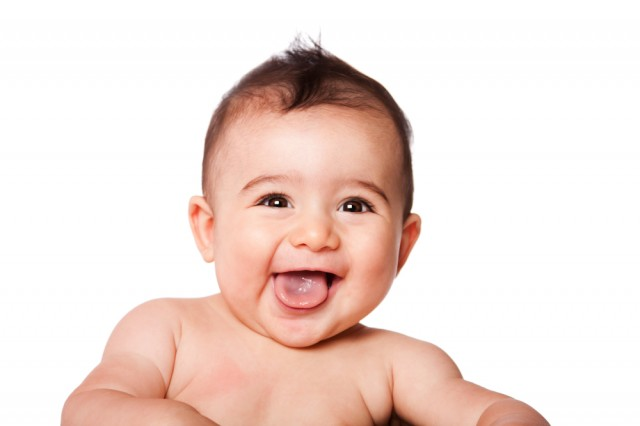
\includegraphics[scale=0.18]{intro/uses/nonverbal1} & 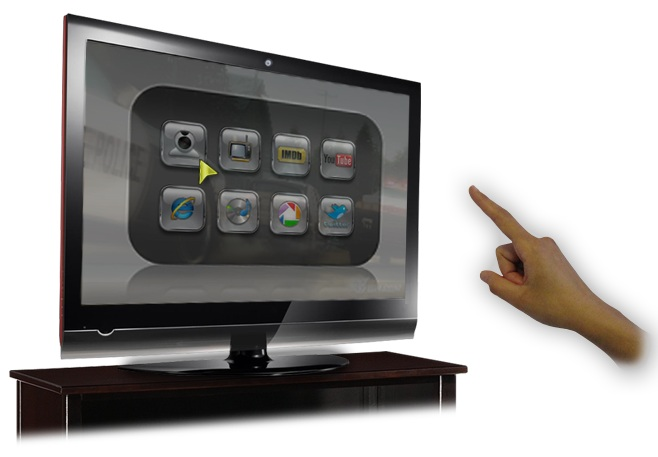
\includegraphics[scale=0.2]{intro/uses/interaction1} \\
La mayor parte de la comunicación es no verbal %\cite{mehrabian1971silent}  
& Método de interacción\\
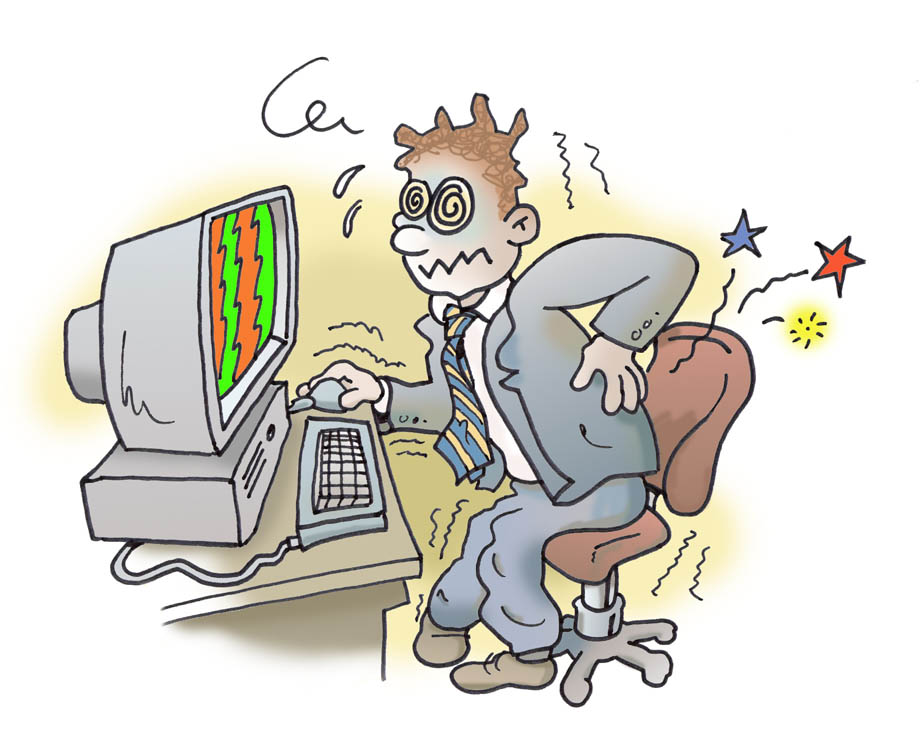
\includegraphics[scale=0.085]{intro/uses/rsi1} & 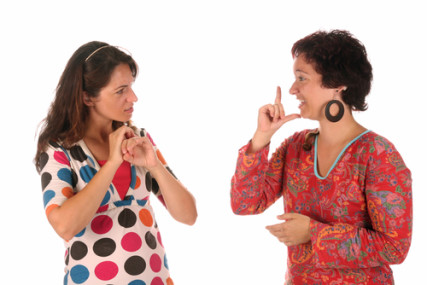
\includegraphics[scale=0.9]{intro/uses/sign_language}\\
Lesiones por sobreuso de PCs %\cite{coggon2013disabling} &  Lenguaje de Señas
\end{tabular}

\begin{block}{}
Existen varios tipos de gestos y formas de reconocimiento. 
\end{block}
\end{frame}


\subsection{Problema}
\begin{myframe}
\frametitle{Descripción del problema}
\begin{columns}
    \begin{column}{0.5\textwidth}
        \begin{itemize}
        \item Reconocimiento de gestos con la mano en 3D
        \item Definidos por el usuario
        \item Pocos gestos para entrenar (3 por cada \textbf{clase de gesto})
        %\item 36 clases (10 dígitos + 26 letras)
        %\item DB de 720 gestos (20 por clase)
        \end{itemize}
    \end{column}
    \begin{column}{0.5\textwidth}
    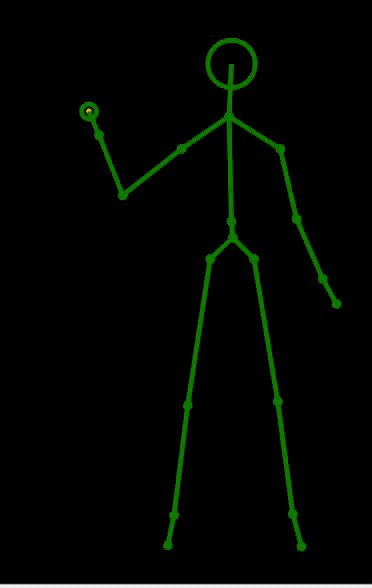
\includegraphics[width=.9\linewidth]{intro/esqueleto}
    \end{column}
  \end{columns}
\end{myframe}


\subsection{Soluciones}


\begin{frame}[fragile]
\frametitle{Modelos explícitos}
  
\begin{exampleblock}{Gesto de saludo}
    \begin{itemize}
          \item La mano comienza debajo del pecho
          \item Subir la mano en línea recta a una velocidad mayor a $V \frac{m}{seg}$
          \item Detener la mano abruptamente arriba de la cabeza
    \end{itemize}      
\end{exampleblock}

\begin{exampleblock}{En GestureML:}
\lstset{breaklines=true,language=XML, tabsize=12}
\begin{center}
\scriptsize
\begin{lstlisting}
<inertial_filter>
  <property ref="drag_dy" active="true" friction="0.9"/>
</inertial_filter>
<delta_filter>
  <property ref="drag_dy" active="true" delta_min="0.5" delta_max="500"/>
</delta_filter>
\end{lstlisting}
\end{center}
\end{exampleblock}
\end{frame}

\begin{myframe}
\frametitle{Modelos generados por Aprendizaje Automático}
\begin{center}
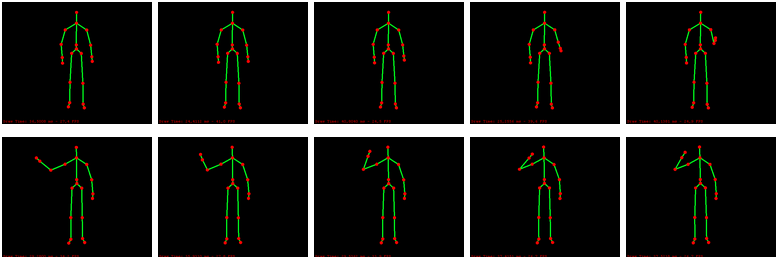
\includegraphics[width=\linewidth]{intro/db}\\
\vspace{15pt}
\arrowdown Entrenamiento \arrowdown \\
\begin{varblock}[3cm]{}
\centering
\huge Modelo
\end{varblock}
\end{center}
\end{myframe}

\begin{myframe}
\frametitle{Modelos Explícitos vs Aprendizaje Automático}
\begin{columns}
    \begin{column}{0.5\textwidth}
        \begin{block}{Definir un modelo \textbf{explícitamente}}
        \begin{itemize}
          \item \textit{Lenguaje de definición de gestos}
          \item Necesita conocimiento experto
          \item Difícil agregar nuevos gestos
          \item Vocabulario limitado
          \item Poco adaptables a distintas personas
        \end{itemize}
        \end{block}
    \end{column}
    \begin{column}{0.5\textwidth}
            \begin{block}{Entrenar un modelo con \textbf{Aprendizaje Automático}}
            \begin{itemize}
              \item \textit{Grabar una base datos de ejemplos para cada tipo de gesto y entrenar un modelo}
              \item Los usuarios pueden grabar nuevos gestos fácilmente
              \item Puede mejorarse automáticamente al usar el sistema
              \item No hay algoritmos de 99.9\% de efectividad
            \end{itemize}
            \end{block}        
    \end{column}
  \end{columns}
\end{myframe}


\begin{frame}
\frametitle{Aprendizaje automático}
\centering
%\esquemaaprendizaje{0.9}
\esquemaclasificacion{0.8}
\end{frame}


\begin{frame}
\frametitle{Entrenamiento + Clasificación}
\centering
   \begin{tabular}{C{0.5\linewidth}C{0.5\linewidth}}
      \uncover<1->{\includegraphics<1->[width=0.5\textwidth]{aprendizaje/ejemplo_entrenamiento1}}
      & \uncover<2->{\includegraphics<2->[width=0.5\textwidth]{aprendizaje/ejemplo_entrenamiento2}}
      \\    
      [-1ex] \uncover<1->{BD} & \uncover<2->{Entrenamiento} \\
      \uncover<3->{ 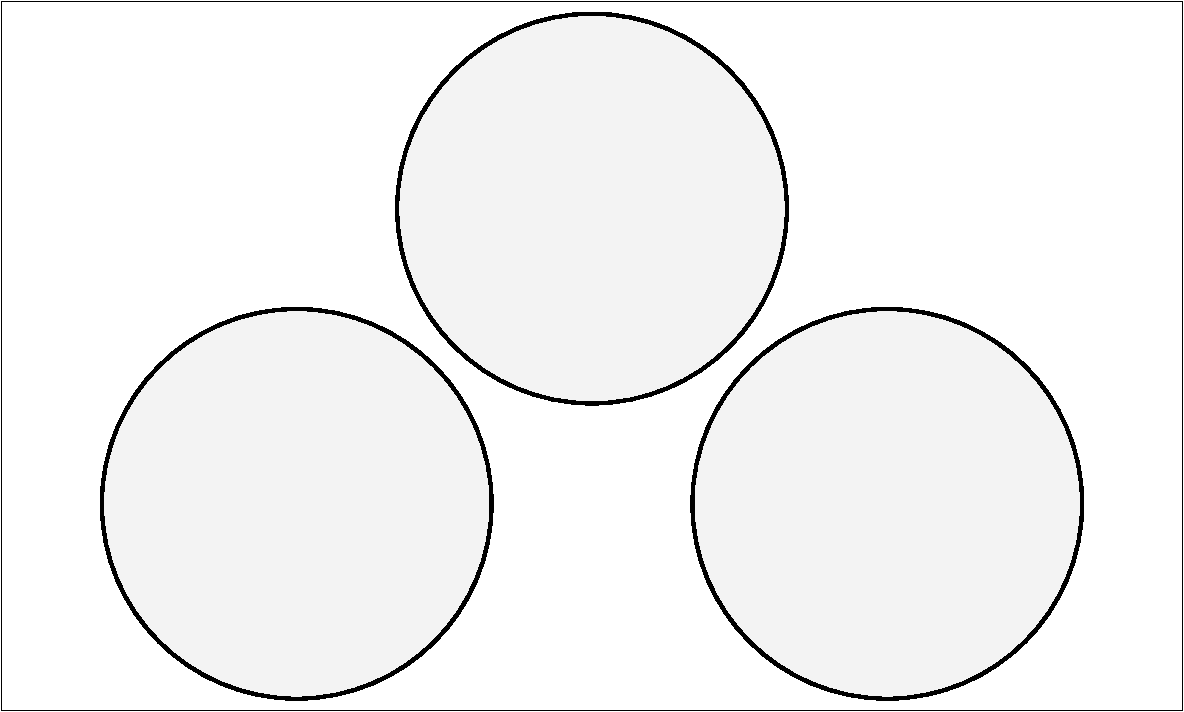
\includegraphics[width=0.5\textwidth]{aprendizaje/model3}}
      & \uncover<4->{ 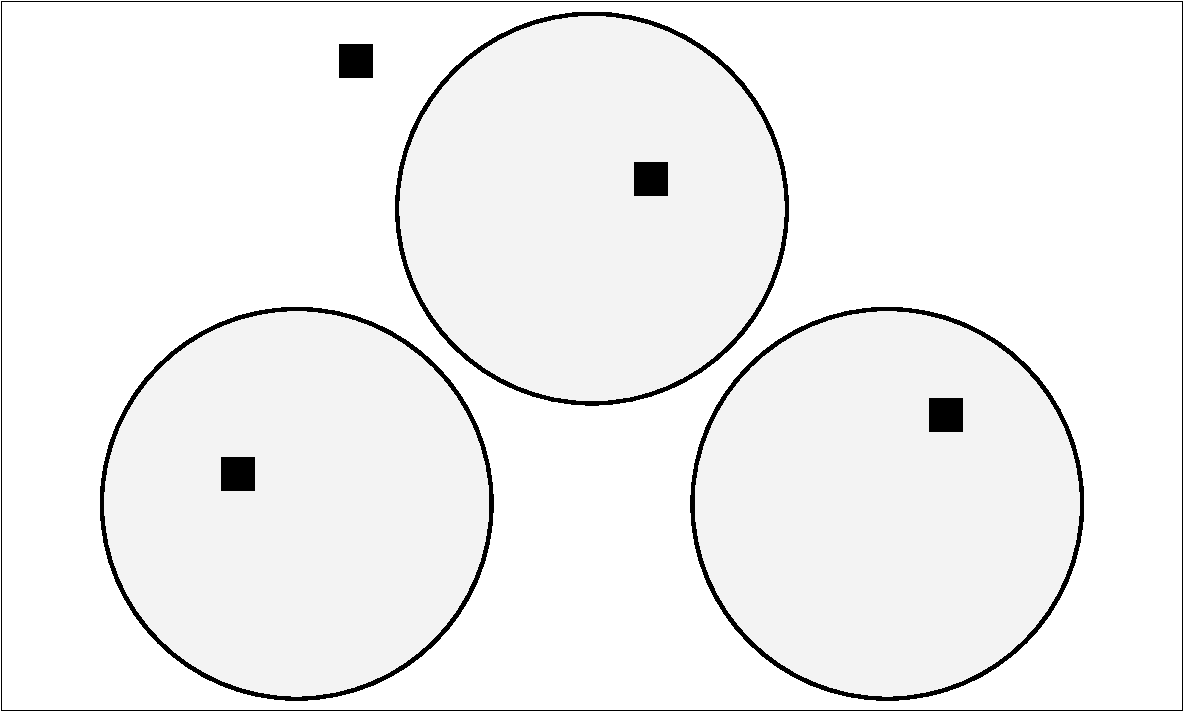
\includegraphics[width=0.5\textwidth]{aprendizaje/new_samples3} }
      \\
      [-1ex]\uncover<3->{Modelo entrenado} & \uncover<4->{Clasificación nuevos gestos}
      \end{tabular}
\end{frame}


\begin{frame}
\frametitle{Trabajo realizado}

\centering
\begin{tabular}{C{0.5\linewidth}C{0.5\linewidth}}
 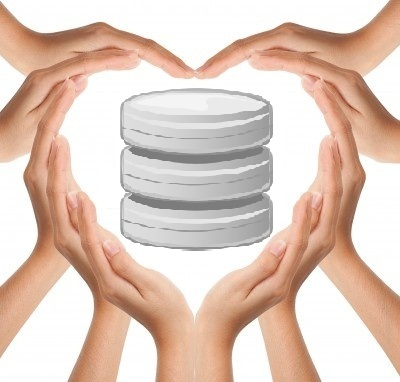
\includegraphics[scale=0.35]{intro/work/hand_db} & 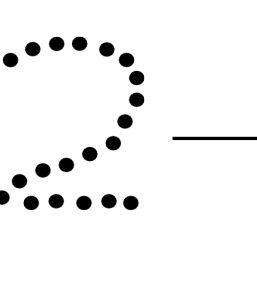
\includegraphics[scale=0.2]{intro/work/representaciones}\\
[-1.5ex] Base de datos de gestos  & Modelo y representaciones de gestos \\
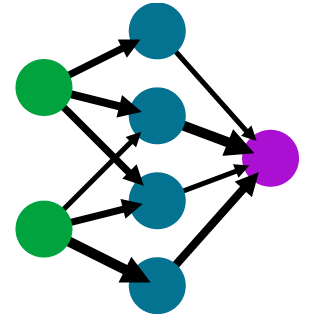
\includegraphics[scale=0.2]{intro/work/cnc} & 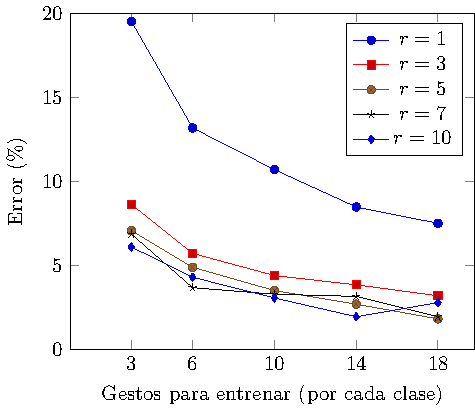
\includegraphics[width=0.34\textwidth]{results/defense_cnc_n} \\  
[-1.5ex] Clasificador Neuronal Competitivo (CNC) & Resultados
\end{tabular}

\end{frame}


%\subsection{}
%\begin{myframe}
%\frametitle{Índice}
%{\small \tableofcontents[hideallsubsections] }
%\end{myframe} 

